% Simplest and effective
% No knowledge of distribution of data
% Instance based learning
% Look at the neighbours to know what you are
% Explain above. Figure
% Performance depends on N and K, also metric
% Some problems regarding increasing and decreasing k

% Classifcation setting.
% Metric gives the measure of dissimilarity


\begin{figure}
    \centering
    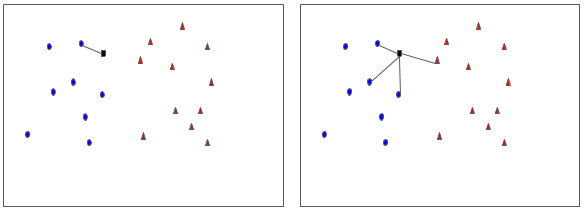
\includegraphics[width=5in, height=1.6in]{concepts/figures/knn.png}
    \caption{Left hand figure shows an example for 1-NN decision rule and the right hand figure shows the example for 4-NN}
    \label{fig:sample_knn_example}
\end{figure}

KNN is one of the simplest and effective classification algorithm used in the community. 
If one doesn't know the distribution of data at hand, it is generally preferred to go 
with KNN as wrong assumption of distribution in other algorithms leads to bad performance.
KNN is an instance based learning or lazy learning as it depends on the samples from a 
small neighbourhood. All the training data is carried over till testing phase, where the 
label of the unknown test data is classified to a label represented by the majority label
of its k-nearest neighbours. Figure~\ref{fig:sample_knn_example} shows the example for labeling the test sample when
K is equal to one and four.

The performance of KNN is dependent on the chosen value of K and also the distance metric
used. The neighbourhood distance of the sample depends on the Kth nearest neighbour. 
Different K results in different distances and different conditional probablities. If value
of K is very small, sample ends up with a small neighbourhood and could result in poor
performance because of data sparseness, noise, ambiguous or poorly labelled data. If we
try to smoothen bad effects by increasing the value of K, it results in introduction of 
outliers from other class and result in over smoothing.

In our experiments, we use KNN in classification setting. Assuming face fiducial detection
is a function given an image, we want to select one best performing function from among the 
functions in the appearance space where we have the training samples. The distance metric 
would give the degree of dissimilarity between the points.
